\chapter{The CMS Experiment at the CERN LHC}

The Large Hadron Collider (LHC) at the European Organization for Nuclear Research (CERN)
is the world's largest and most powerful particle collider.~\cite{Evans:2008zzb} It collides protons 
at a center of mass energy of $13\TeV$, and lead ions at $2.76\TeV$ per nucleon.
Collisions of protons at the LHC are the sole focus of this thesis. 
The protons or ions are brought to collision at the center of four large detectors,
themselves a combination of many detector technologies. 
The particle detectors at the LHC were conceived, developed, and constructed over decades
by collaborations of thousands of scientists from hundreds of nations to
achieve a broad program of research. The detectors were designed and are operator 
by mutually exclusive collaborations of scientists working independently,

The detector sites are

\begin{itemize}
  \item A Large Ion Collider Experiment (ALICE) detector, located at access point 2.
  Designed for the study of lead-ion collisions, especially for the characterization
    of quark gluon plasmas formed in collisions.~\cite{Aamodt:2008zz}
  \item A Large Toroidal LHC ApparatuS (ATLAS) detector, located at access point 1.
  A general purpose detector. Designed for sensitivity to new physics
  with decays to stable SM particles, in particular the 
    discovery and characterization of the SM Higgs boson.~\cite{Aad:2008zzm}
  \item The Compact Muon Solenoid (CMS) detector, located at access point 5.
    A general purpose detector with comparable measurement potential to the ATLAS detector.~\cite{Chatrchyan:2008aa}
  \item The Large Hadron Collider Beauty (LHCb) detector, located at access point 8.
  Designed to characterize the production and decay of b-quark hadrons. Particularly
    focused on CP violation in these decays.~\cite{Alves:2008zz}
\end{itemize}

Results in this thesis are based on an analysis of proton--proton collisions at the LHC 
collected by the CMS detector in 2016. This chapter describes the design principles of the 
LHC and the CMS detector, as well as their operating characteristics in 2016.
  
\section{The Large Hadron Collider}
The LHC was proposed to the CERN council, the management group of the 
laboratory, in 1994, and accepted
with a preliminary budget in 1995. Construction was initially completed in
2008, with full operation beginning in 2009 after setbacks 
encountered in the initial commissioning.
The collider is located on the outskirts
of Geneva, Switzerland and in the nearby French countryside,
which has been the site of the CERN laboratory since it was founded in 1954.
The project was funded by the 20 member states of CERN, as well
as monetary and research contributions from many other nations participating 
in the project, including the United States.

The principle design considerations of a particle collider are the energy
of the particle collisions, the rate of collisions, and the objects collided.
The collided objects determine the possible interactions which can be probed,
while the energy of the collision drives the mass range which can be probed,
given that the produced particle mass $m$ be less than the 
center of mass energy. As particle interactions are quantum mechanical 
and fundamentally stochastic in nature, the rate of collisions is also 
critical for achieving statistically significant measurements.

Several characteristics of proton--proton collisions motivated the decision 
to use protons in the world's highest-energy collisions. Existing high-energy
accelerators, notably the Large Electron Positron Collider (LEP) collider
at CERN and the Tevatron collider at Fermilab in the United States, collided
particle--antiparticle pairs. This is advantageous for processes which proceed by annihilation, 
but requires production of positrons or antiprotons, which is a significantly
bottleneck on achieving a high rate of collisions. 

The LHC is situated in a $26.7\unit{km}$ tunnel, $45$--$170\unit{m}$
below the Swiss and French country side. The tunnel pre-dates the LHC,
having been originally built for the Large Electron Positron (LEP) collider.
It consists of 8 straight sections $528\unit{m}$ in length, and 8 arced sections.
The majority of the tunnel is $3.7\unit{m}$ in diameter, with larger excavated
areas at the four experimental caverns and other access points.
The primary motivation for an underground tunnel is to circumvent the high
cost of land acquisition, but underground operation is also advantageous for
reducing the cosmic radiation reaching the experimental cavern and  
for shielding the radiation produced by the LHC.

The protons are directed through pipes inside the tunnel, which are held
at high vacuum. The positions and accelerations of the protons are controlled 
by magnetic and electric fields maintained by instrumentation surrounding the 
vacuum pipes. The arced sections are equipped with dipole magnets,
which direct charged objects along a circular path.
The size of the LEP tunnel prohibited the installation of two independent beam
systems, which led to the adoption of a unique "two-in-one" superconducting
magnet design~\cite{}, shown in Fig~\ref{fig:dipoleXsec}. 

\begin{figure}[htbp]
  \centering
   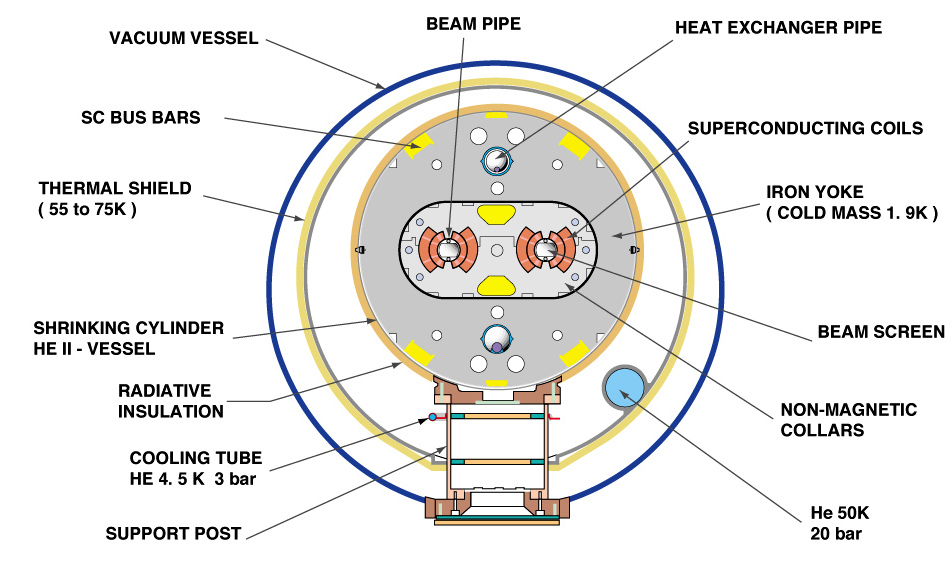
\includegraphics[width=\textwidth]{figures/LHCandCMS/dipoleXSec.jpeg}
  \caption{
    Cross section of an LHC dipole magnet~\cite{Jean-Luc:841539}.
        }
 \label{fig:dipoleXsec}
\end{figure}

Neglecting synchrotron radiation,
the primary limitations on the energy of a synchrotron come
from the magnetic field of the bending magnets and the radius of curvature
of the tunnel. For an particle of charge $q$ with velocity $v$ accelerated at
in a circular 
trajectory of radius $R$ trough a magnetic field of strength $B$
The energy $E$ of the particle is given by

\begin{equation}
  E = eBRv \approx qBRc \,,
\label{eq:beamEnergy}
\end{equation}

where $v \approx c$, the speed of light, for $p \gg m$. Increasing the radius
requires a larger tunnel, which is limited by the cost of construction. 
The LHC tunnel size was set by the existing LEP tunnel, so achieving
a sufficient magnetic field was a major focus of the LHC development. 

Dipole magnets with a maximum field strength of $8.33\unit{T}$ were achieved
at an affordable cost through major technological advances. Such a high 
field necessitates the use of superconducting magnets. The magnets 
are constructed of niobium-titanium, and are operated at $1.9\unit{K}$,
lower than any previous accelerator. 
at 
first accelerator to operate 
In particular,
the LHC is the first accelerator to operate 
Because about 80\% of the arced sectors of the LHC are equipped with dipole magnets,
the bending radius of the dipoles is $2.804\unit{km}$, yielding the design energy
of $7\TeV$ per beam from Equation~\ref{eq:beamEnergy}.

Also brief mention of the 

How it accelerates protons (e.g., the system of accelerators)

The magnet design and characteristics 

The RF and bunch characteristics

Focusing beams to collisions


\section{Operation of the LHC in 2016}
\section{The Compact Muon Solenoid experiment}

The CMS detector is a general-purpose detector designed to 
study particle production and interactions at the TeV scale.
A major design principle of the CMS detector was the ability to 
probe the nature of electroweak symmetry breaking, which has been
achieved through the discovery and characterisation of a scalar boson
consistent with the SM Higgs boson~\cite{}. The design of the CMS detector
ensured sensitivity to a Higgs boson with mass up to
$1\TeV$ in its SM decays, as well as sensitivity to a broad class
of BSM theories. In terms of detector performance, these design principles,
as defined in Ref.~\cite{Chatrchyan:2008aa}, are:

\begin{itemize}
  \item Accurate mmuon identification and high momentum resolution, including
    dimuon mass resolution of $\approx 1\%$ at $m_{\mu\mu} = 100\GeV$ and correct charge
    assignment up to $\pt^{\mu}\approx 1\TeV$.
  \item Identification of objects with a short but significantly decay time,
    including tau leptons and b hadrons, which requires fine position resolution 
    close to the interaction point to distinguish their displaced tracks.
  \item Good electromagnetic energy and momentum resolution, achieving
    diphoton and dielectron mass resolution of $\approx 1\%$ at $m_{ee} = 100\GeV$,
    and sufficient granularity to distinguish prompt diphotons from $\pi^{0}$ decays to photons.
  \item Sufficient calorimeter resolution and hermeticity for precise dijet mass
    and missing transverse momentum reconstruction.
\end{itemize}

The CMS detector has a cylindrical geometry. As shown in Fig.~\ref{fig:CMScutaway},
it is built from the combination
of several detector technologies which work in harmony to achieve the outlined design
goals. The following sections briefly describe each of the detector subsystems
which comprise the CMS detector. 
Chapter~\ref{ch:reconstruction} details the ways in which these subsystems 
are used together to reconstruct the physics objects used for the results
presented in this thesis.

\begin{figure}[htbp]
  \centering
   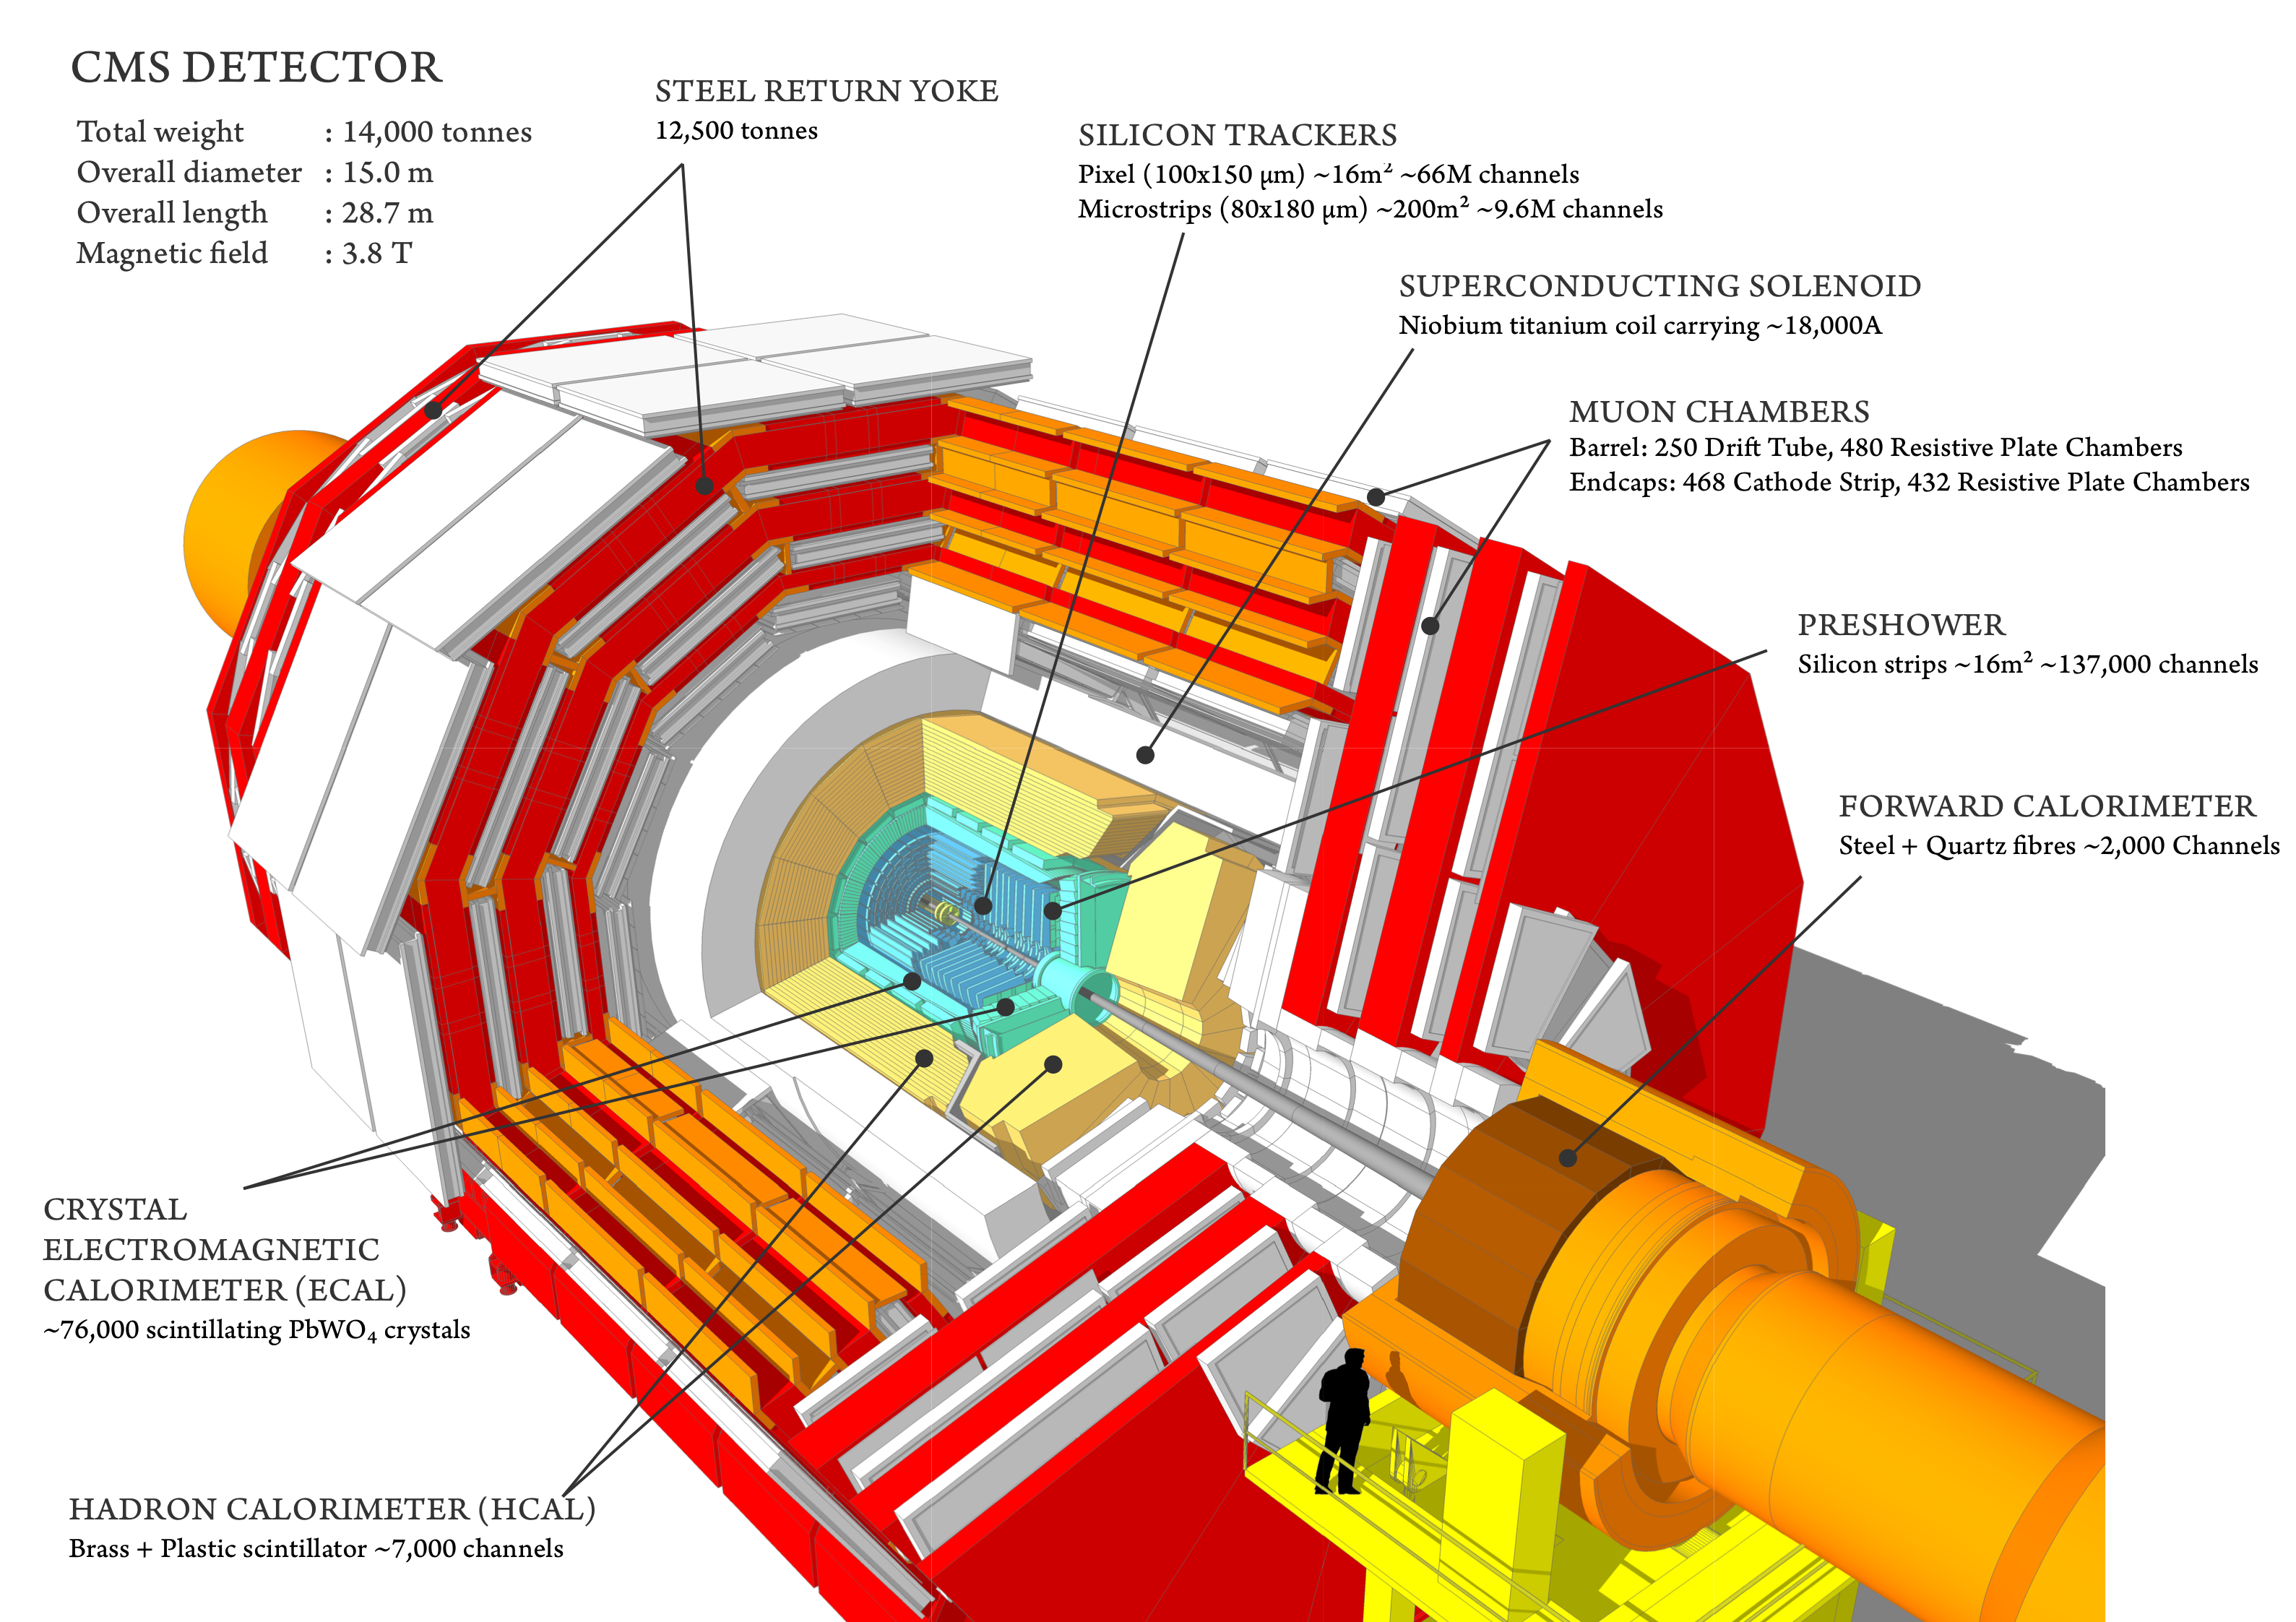
\includegraphics[width=\textwidth]{figures/LHCandCMS/CMScutaway.png}
  \caption{
    A cutaway view of the CMS detector, showing each detector 
    subsystem~\cite{1742-6596-513-2-022032}.
        }
 \label{fig:CMScutaway}
\end{figure}

The coordinate system adopted by CMS, and used in this thesis,
is a right-handed coordinate system with the point $(x, y, z) = (0, 0, 0)$
centered in the detector, at the nominal collision point. The $y$-axis 
is perpendicular to the earth, where vertically upward defines the $+y$ direction.
The $x$-axis is in the plane of the LHC, with the $+x$ direction pointing towards
the center of the ring. The $z$-axis points through the center of the detector
along the direction of travel of the colliding protons, where $+z$ is defined
by the right-handedness of the coordinate system. In polar coordinates, 
the azimuthal angle $\phi$ is measured from the $x$-axis in the $x$-$y$
plane, and the polar angle $\theta$ is measured from the $z$-axis. The radial
coordinate $r$ is defined as $r = \sqrt{x^2 + y^2 + z^2}$.
Because the production of 
particles is preferentially in the forward direction (along
the $z$-axis), it is convenient to introduce the pseduorapidity $\eta = - \ln(\tan{\theta/2})$
for the polar coordinate. The momentum in the transverse direction,
defined as $\pt = \sqrt{p_{x}^2 + p_{y}^2}$, is a particularly important quantity.
because the initial transverse momentum of the collision is zero.
In this thesis, the four-momentum of an object will commonly be expressed as
$p = p(m, \vec{p}) = p(m, \pt, \eta, \phi)$.

\section{The CMS solenoidal magnet}

The central feature of the CMS apparatus is a superconducting solenoid 
of $6\unit{m}$ internal diameter and $12.5\unit{m}$ in length,
constructed from 4 layers of reinforced niobium titanium.
It provides a nearly constant $3.8\unit{T}$ magnetic field inside the solenoidal volume.
The magnetic flux of the solenoid is returned through
a $12 000$-tonne steel yoke, comprising 5 wheels and 2 endcaps,
which is fully saturated to approximately $2\unit{T}$. 
The tracker and calorimeters are situated inside the solenoid, while 
the muon detectors are embedded in the steel return yoke, as shown
in Fig.~\ref{fig:CMScutaway}.

During operation, the CMS solenoid stores approximately $2.4\unit{GJ}$ of 
energy, the largest magnet in the world by this metric. This immense
size leads to a powerful bending radius for charged objects within the detector,
which is a critical metric for particle reconstruction and identification.
In particular, objects of charge $q$ moving
in a magnetic field $\vec{B}$ at velocity $\vec{v}$ experience a Lorentz force,

\begin{equation}
  \vec{F} = q\vec{B} \times \vec{v} \,.
\end{equation}

Because the solenoidal field is constant and aligned along the $z$-direction, 
$\vec{B} = B\hat{z}$, the force is purely in the transverse direction.
Consequently, charged particles within the CMS
solenoid travel along a nearly helical path of radius $R=\pt/\abs{q}B$, where 
small deviations from this path arise from non-uniformity of the field
and interactions in the detector material. The sign of a 
$\pt$ of a particle of known charge can therefore be deduced by measuring its radius of
curvature. The bending power of the magnet $BR$ is therefore a critical 
parameter determining the detector capability for accurate particle $\pt$ measurement.
The nearly $12\unit{Tm}$ bending power achieved by the CMS is critical to achieving
the high momentum resolution outlined in the design goals of the experiment. It
is also fundamental to the particle flow reconstruction technique utilized by CMS,
outlined in Chapter~\ref{ch:reconstruction}.

\section{The CMS silicon tracking system}

Stuff about this

\section{The CMS electromagnetic calorimeter}
\section{The CMS hadronic calorimeter}
\section{The CMS muon system}

As suggested by the CMS name itself, the muon detector subsystem is essential to the
achieving the experimental goals of the CMS experiment. 
High-energy muons are produced in many heavy-object SM and BSM 
decays, and long-established detector technologies are well suited to muon detection in LHC collisions.
Muons with $v\approx c$ are nearly stable
on timescale of the traversal of the CMS detector volume. As the heavies stable lepton, 
they are less susceptible to electromagnetic radiative energy loss than electrons, and therefore
interact minimally with the calorimeter system. Detector technologies suitable for
charged-particle detection, placed outside all other detector systems, 
are therefore ideal for muon detection. 

\begin{figure}[htbp]
  \centering
   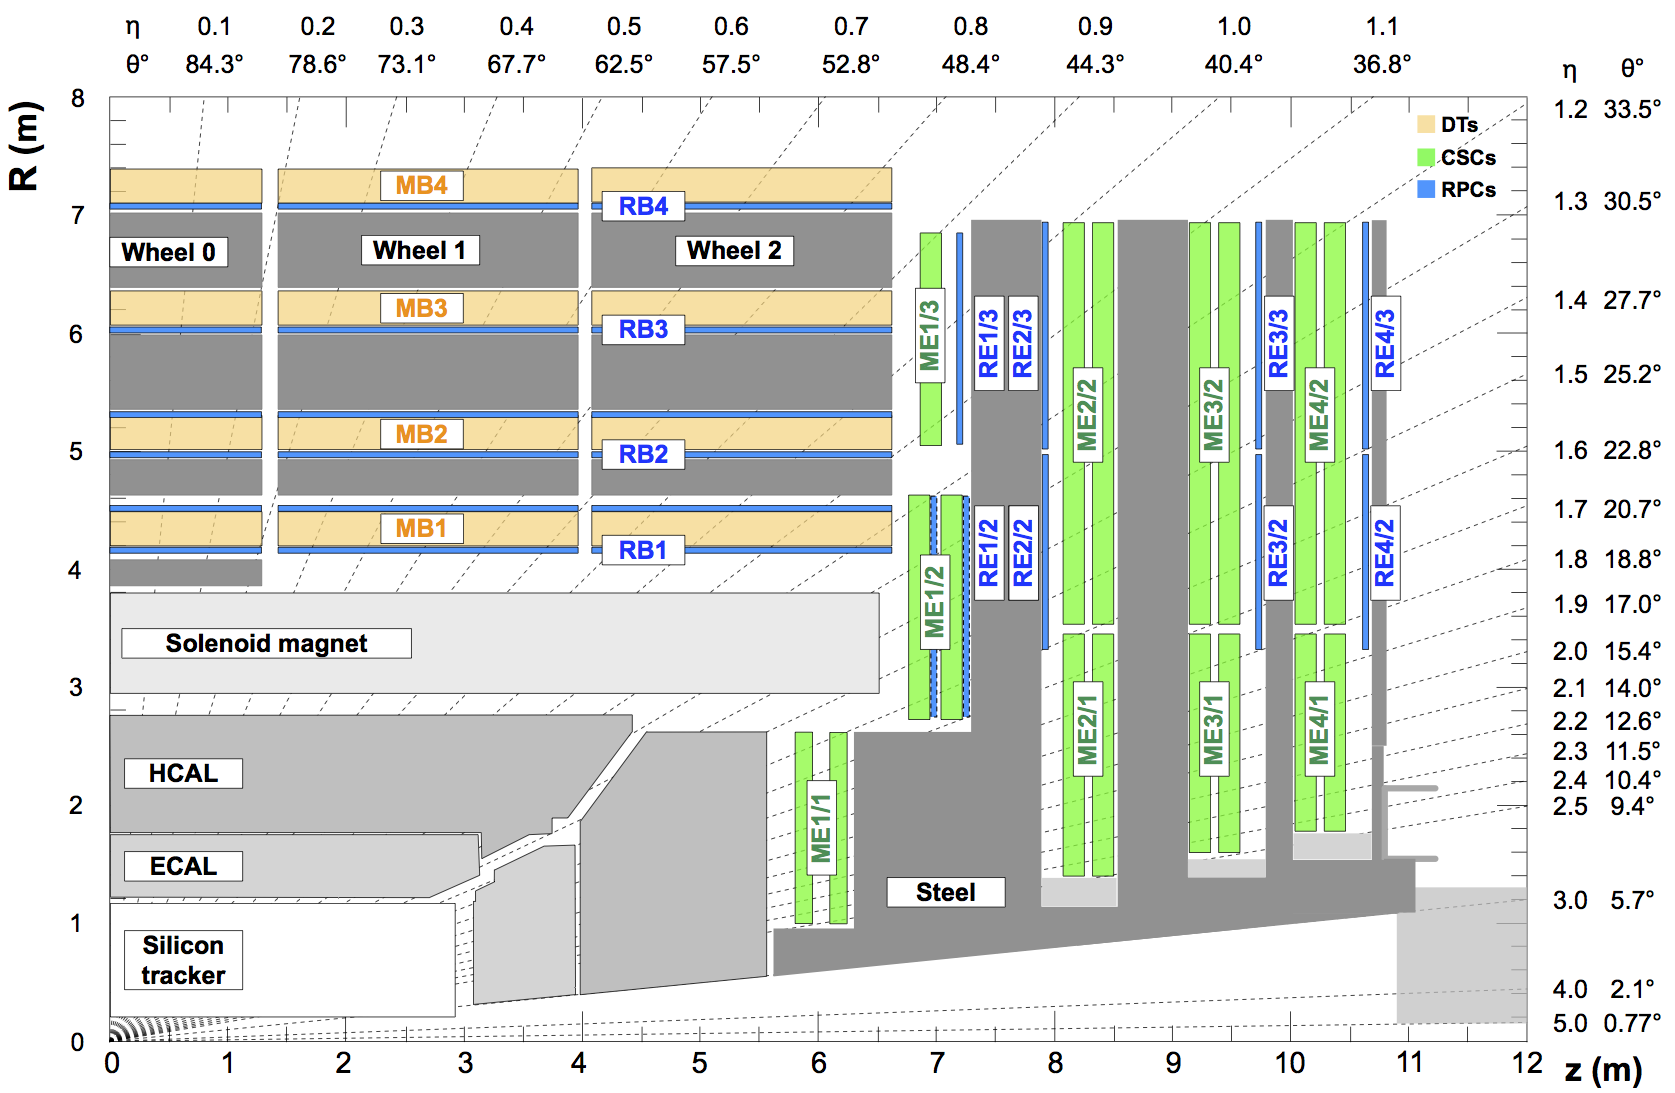
\includegraphics[width=\textwidth]{figures/LHCandCMS/MuonSystemGeometry.png}
  \caption{
    An $R-z$ cross section of a quadrant of the CMS detector, with the interaction
    point at the bottom left corner. The locations of the detectors
    comprising the CMS muon system within the steel steel return yoke
    are shown~\cite{Chatrchyan:2012xdj}.
        }
 \label{fig:muonSystemGeo}
\end{figure}

The muon system is composed of three technologies, 
described in more detail in the following sections. 
Each operates on the principle of gas ionization. 
The detectors consist of a volume of 
gas over which an electric field is applied. Charged
particles passing through the volume ionize the gas, and the ionized gas molecules
and free electrons drift in the electric field towards read-out electronics at the 
edges of the detector volume. The track of the interacting object is inferred from
the position and timing of the measured electrons and ions.
The operating characteristics of the gas ionization detectors can be modified
for fast readout, high granularity, and 
In the CMS detector, these considerations, along with the cost of construction 
for detectors covering an area of $\\approx 25,000\unit{m}^2$ and 
the effect of the radiation environment of the detector on performance, motivate
the specific design choices.

Gas ionization detectors are
sensitive to all charged particles passing through the detector. As previously discussed,
nd illustrated in Fig.~\ref{fig:muonSystemGeo}, the muon system is 
the outer layer of the CMS detector, embedded in
the steel return yoke of the magnet system. This structure, along with the inner
detector systems, serves as shielding for the muon system and ensures that the 
well over 99\% of objects reaching the muon system are muons.

\subsection{Drift tube system}

The barrel part of the muon detector, $\abs{\eta} < 1.2$,
is composed of drift tube (DT) chambers. In this region, the magnetic field
outside the return yoke is generally small (below 0.2\unit{T}), and the muon occupancy is low, justifying
the use of DT detectors. The DT system is built from individual DTs, 
rectangular aluminum tubes with a length of 2.4\unit{m} and a cross section
of $13\times42\unit{mm}^2$, shown in Fig~\ref{fig:DTs}. At the center of each
tube is a 50-\micron-diameter gold-plated stainless-steel anode wire.
Aluminum strips are attached to the interior of the aluminum 
structure---insulated by mylar tape---to
shape the electric field to the pattern illustrated in Fig.~\ref{fig:DTs},
and an 85\% Ar 15\% CO$_2$ gas mixture is contained in the volume. 
The drift time for muons crossing a
cell at a maximum distance from the anode wire of 21\unit{mm}
is about 380\micron, which is sufficient to keep the occupancy low.
Muons passing through the gas volume ionize the gas and create an avalanche of
electrons around the very high field at the anode wire.
A time-to-digital converter reads out the electrical pulse of the electrons.
The arrival time of the signal, corrected by the drift velocity and the time
from the collisions to the trigger decision, are used to obtain the muon interaction
position. 

\begin{figure}[htbp]
  \centering
   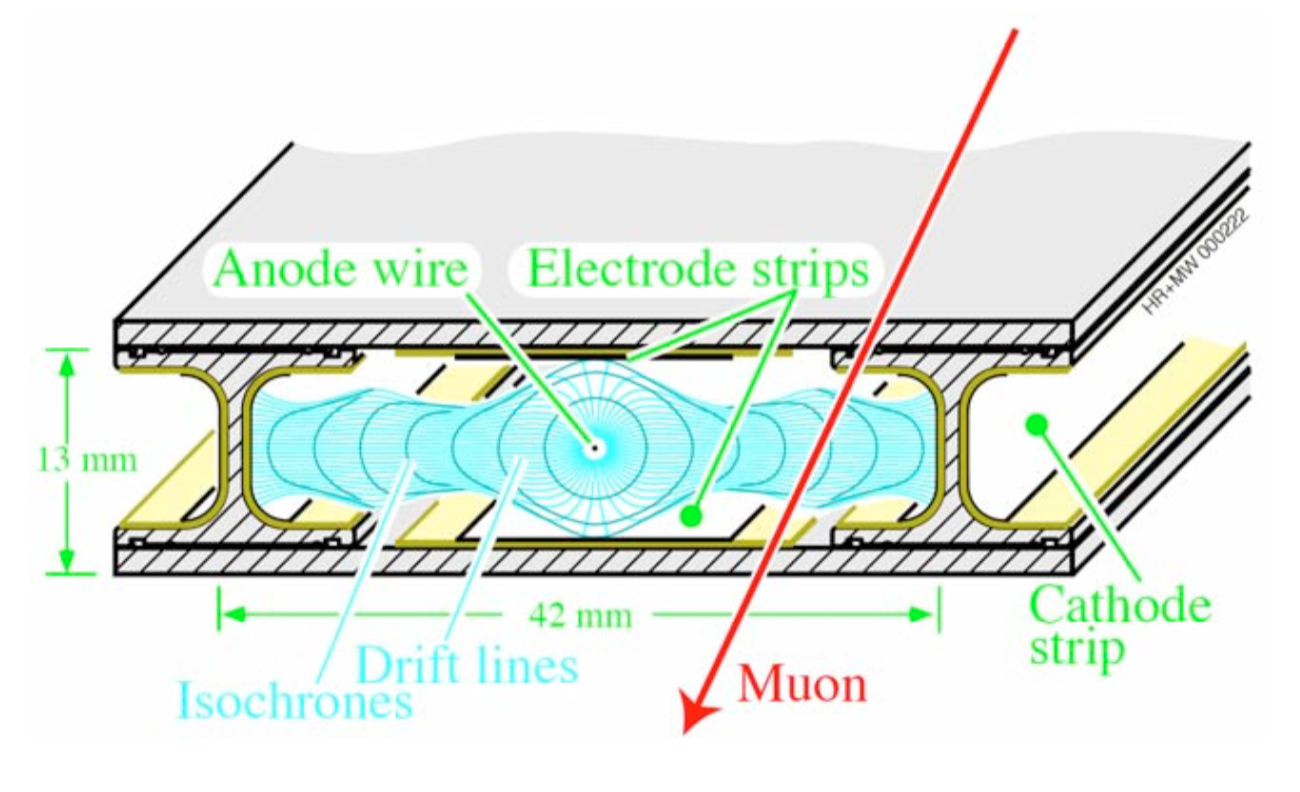
\includegraphics[width=0.6\textwidth]{figures/LHCandCMS/DriftTubeCutaway.png}
  \caption{
    Diagram of a drift tube cell, from Ref.~\cite{}. The 
    geometry of the cell and the electric field lines resulting from the 
    anode wire and electrode strips are illustrated.
        }
 \label{fig:DTs}
\end{figure}


The DT cells are assembled into superlayers (SL), composed of 
4 layers of drift cells staggered by half a cell. 
The SLs are grouped into chambers of 2 or 3 SLs which are arranged into stations
within the magnet return yoke.
The wires in the outer SLs within a chamber are parallel to beam line, providing
a measurement in the bending plane.
An additional inner SL is aligned perpendicular to the beam direction, 
for all chambers but those in the 
outermost station, to provide a measurement in the $z$ plane. 
The chambers are arranged in concentric cylinders
around the beam line, with 60 chambers each in the three inner cylinders
and 70 in the outer cylinder. In total there are $\approx172,000$ 
cells, read out as independent channels. The offset arrangement of the cells
eliminates dead spots in the efficiency, and allows a measurement of the
muon crossing time to be obtained using meantimer circuits.
The muon position resolution in the DTs is around 100\micron and the
timing resolution is within a few ns.

\subsection{Cathode strip chamber system}

Cathode strip chambers (CSC) are used in
the forward regions of the CMS detector ($0.9 < \abs{eta} 2.4$), 
where the prompt and background muon rates are high, and the magnetic field
is large and non-uniform.

\subsection{Resistive plate chamber system}

A crucial role of the muon system is to provide muon position and momentum
measurements in a sufficiently timescale
to determine if an event justifies storage offline analysis. 
This process, known as event triggering,
is described in additional detail in Section~\ref{sec:triggering}.
While the DT and CSC system provide fast readout, the background rate and
importance of associating an event with the correct bunch crossing (within
25\unit{ns}) make additional redundancy desirable.

A system of resistive plate chambers (RPC) in both the barrel and endcap
($\abs{\eta} < 1.2$ accomplishes this goal. The RPCs are double-gap chambers
constructed from a thin layer of readout strips between two electrodes held 
at high voltage, forming a volume filled predominately with C$_2$H$_2$F$_4$ gas.
The system is operated in avalanche mode, where the sum of the signals
in the two gaps created by an interacting muon is read out on strips
at the center plate. The plates are separated by 2\unit{mm}, which ensures
that the charge avalanche is observed well below the 25\unit{ns} window
needed to assign the muon to the correct bunch crossing.
There are 6 layers of RPCs in the detector barrel, interspersed among the DTs,
and 3 layers in the endcap alongside the CSCs. The readout strips in the barrel RPCs
subtend an angle of 5/16 degree. The position resolution of the RPCs, about 1\cm,
is below the DT and CSC systems, but the system provides an independent position
and timing measurement. 

\section{Data triggering and acquisition}
\label{sec:triggering}
\section{Luminosity measurement}
